%=====================================================================
% From Cain to Matignon
% Submission manuscript — Mathematics / MDPI template
%=====================================================================
\documentclass[mathematics,article,submit,pdftex,moreauthors]{../reference-paper/Definitions/mdpi}

\usepackage{amsmath,amssymb,amsthm,mathtools}
\usepackage[none]{hyphenat}

\DeclareMathOperator{\spec}{spec}
\DeclareMathOperator{\diag}{diag}
\DeclareMathOperator{\Real}{Re}
\newcommand{\R}{\mathbb{R}}
\newcommand{\C}{\mathbb{C}}
\newcommand{\Falpha}{\mathcal{F}_{\alpha}}
\newcommand{\Palpha}{\mathcal{P}_{\alpha}}
\newcommand{\Salpha}{\Sigma_{\alpha}}
\newcommand{\Dpos}{D\succ0}
\newcommand{\CapD}[1]{{}^{C}\!D_t^{#1}}

\graphicspath{{../computations/figures_wave2/exports/pdf/}{../computations/figures/exports/pdf/}}

\firstpage{1}
\makeatletter
\setcounter{page}{\@firstpage}
\makeatother
\pubvolume{1}
\issuenum{1}
\articlenumber{0}
\pubyear{2026}
\copyrightyear{2026}
\hreflink{https://doi.org/}

\Title{From Cain to Matignon: Exact Positive-Diagonal Stability in Dimension Three and a Nonlinear Caputo Ecological Realization}

\Author{{Ibrahim Alraddadi}$^{1}$ and Thoraya N. Alharthi $^{2,*}$}
\AuthorNames{Ibrahim Alraddadi and Thoraya N. Alharthi}

\address{%
$^{1}$ \quad Department of Mathematics, Faculty of Science, Islamic University of Madinah, Madinah 42351, Saudi Arabia; ialraddadi@iu.edu.sa\\
$^{2}$ \quad Department of Mathematics, College of Science, University of Bisha, P.O. Box 551, Bisha 61922, Saudi Arabia}

\corres{Correspondence: talhrthe@ub.edu.sa}

\abstract{Positive-diagonal \(D\)-stability asks whether stability persists under every positive diagonal left scaling. We replace the classical Hurwitz half-plane by the Matignon sector for commensurate Caputo systems and solve the resulting real three-dimensional problem on the full-dimensional strict-\(P(-A)\) stratum. Four scale-invariant quantities \((\beta_{12},\beta_{13},\beta_{23},\kappa)\) reduce the complete positive-diagonal orbit to an open simplex, and for \(2/3<\alpha<1\) we prove the exact criterion \(\kappa<T_{\alpha}(\beta)\). At \(\alpha=1\), \(T_{\alpha}\) collapses to Cain's classical threshold, while \(T_{\alpha}>T_1\) for every \(\alpha<1\), producing an explicit genuinely fractional band. The threshold objective is strictly convex in logit coordinates, has a unique nondegenerate optimizer, and yields the minimum-dimension result: three is the first dimension in which the genuinely fractional multiplicative-\(D\)-stable class has nonempty full-dimensional interior. We then construct a nonlinear three-species Caputo Kolmogorov realization with double-Allee basal growth and intraguild predation. A natural competing-consumer architecture is proved unable to enter the fractional-only band, whereas the intraguild-predation architecture realizes an open biological subset of it. Finally, varying only the Allee threshold moves the fixed biological system transversally across Cain's classical \(D\)-stability boundary into the fractional-only Matignon region.}

\keyword{fractional-order systems; Caputo derivative; D-stability; Matignon stability; P-matrix; Cain criterion; intraguild predation; double Allee effect; ecological stability}
\MSC{15A18; 34A08; 34D20; 92D25}

\begin{document}

\section{Introduction}\label{sec:introduction}

Stability under a single Jacobian is often too weak a robustness requirement. In matrix \(D\)-stability one asks instead whether the spectrum remains in a prescribed stability region after \emph{every} positive diagonal left scaling. For the classical Hurwitz half-plane this problem has a long history, with exact low-dimensional results, interior and strong-\(D\)-stability theory, and structural criteria based on principal minors and feedback cycles \cite{Cain1976,BahlCain1977,Hartfiel1980,Cain1984,Abed1986,LeeEdgar2001,Kushel2019}. The question addressed here is what becomes of this all-diagonal robustness requirement when the underlying dynamics are commensurate fractional-order systems.

For a Caputo system of order \(0<\alpha<1\), asymptotic stability of the linearization is governed by the Matignon sector rather than the open left half-plane: every eigenvalue must satisfy
\[
 |\arg \lambda|>\frac{\alpha\pi}{2}.
\]
We use the original proceedings formulation together with a modern published treatment of Caputo stability \cite{Matignon1996,BrandiburGarrappaKaslik2021}. For \(\alpha<1\), the Matignon region strictly contains the left half-plane, so an equilibrium may be fractionally stable even when a conjugate pair has positive real part. This familiar fixed-matrix phenomenon is not our novelty; it is the geometric reason a fractional analogue of multiplicative \(D\)-stability can differ from the classical one.

Generalized matrix stability with respect to spectral regions and multiplier classes is already established. In particular, Kushel's unifying framework includes multiplicative positive-diagonal actions, and Kushel and Pavani give forbidden-boundary criteria for generalized \(D\)-stability in unbounded LMI regions, including conic sectors and their complements \cite{Kushel2019,KushelPavaniJDDE,KushelPavani2021,Kushel2023}. Thus the problem considered here is \emph{not} the first necessary-and-sufficient formulation of generalized \(D\)-stability. Our contribution is lower-dimensional and explicit: for real \(3\times3\) matrices on the full-dimensional strict-\(P(-A)\) stratum, we eliminate the entire positive-diagonal multiplier orbit and reduce the Matignon condition to a scalar threshold in four invariant coordinates.

The classical endpoint of this construction is equally important. Cain's exact criterion for real \(3\times3\) \(D\)-stable matrices already shows that principal minors, homogeneity in the diagonal multiplier, and an exact minimization over the multiplier orbit are classical ingredients \cite{Cain1976}. The present threshold should therefore be read as a fractional deformation of Cain's boundary, not as an unrelated sufficient test. Other adjacent theories are also occupied: P-matrix eigenvalue wedges \cite{Kellogg1972}, fixed-polynomial fractional Routh--Hurwitz criteria \cite{CermakNechvatal2017,BourafaAbdelouahabMoussaoui2020}, forbidden-sector polynomial results \cite{HoltzKhrushchevKushel2016,JoyaFuruta1991}, and structured cyclic fractional-network conditions \cite{Siami2021}. The exact arbitrary-\(\beta\) all-diagonal threshold derived below is not implied by any of these results.

The first structural result is dimensional. In dimension two we obtain the exact classification
\[
 A\in\mathcal F_\alpha^{(2)}
 \iff
 \det A>0,\qquad a_{11}\le0,\qquad a_{22}\le0,
\]
and the genuinely fractional difference from classical \(D\)-stability lies only on a codimension-two diagonal-equality set. Hence it has empty full-dimensional interior. In dimension three the situation changes qualitatively. On the strict-\(P(-A)\) stratum, four normalized principal-minor invariants
\[
 (\beta_{12},\beta_{13},\beta_{23},\kappa)
\]
encode the positive-diagonal orbit. For \(2/3<\alpha<1\) we prove
\[
 A\in\mathcal F_\alpha^{(3)}
 \iff
 \kappa<T_\alpha(\beta),
\]
where \(T_\alpha\) is an exact two-dimensional simplex minimum. At \(\alpha=1\),
\[
 T_1(\beta)
 =
 \left(
 \sqrt{\beta_{12}}+
 \sqrt{\beta_{13}}+
 \sqrt{\beta_{23}}
 \right)^2,
\]
which is Cain's classical boundary. For every \(2/3<\alpha<1\),
\[
 T_\alpha(\beta)>T_1(\beta),
\]
so
\[
 T_1(\beta)<\kappa<T_\alpha(\beta)
\]
is an open, genuinely fractional, all-positive-diagonal stability band. For \(0<\alpha\le2/3\), Kellogg's P-matrix wedge gives the complementary low-order characterization. Together with the exact two-dimensional obstruction, this yields
\[
 \min\left\{
 n:
 \operatorname{int}
 \left(
 \mathcal F_\alpha^{(n)}
 \setminus
 \mathcal D_H^{(n)}
 \right)
 \ne\varnothing
 \right\}=3
 \qquad
 \forall\,0<\alpha<1.
\]

The threshold is not merely an implicit minimum. Its logarithm is globally strictly convex in logit coordinates, giving a unique nondegenerate optimizer and smooth parameter dependence. It decreases strictly with \(\alpha\) and approaches Cain's surface linearly as \(\alpha\to1^{-}\); Siami's cyclic condition is recovered as the fully symmetric slice \(\beta_{12}=\beta_{13}=\beta_{23}=1\) \cite{Siami2021}.

We next ask whether the exact difference band is only an abstract matrix phenomenon. Classical ecological \(D\)-stability is established \cite{HouBaigent2015,ChenWangLiu2024}; IGP and IGP with Allee effects are standard motifs \cite{HoltPolis1997,BaiKangRuanWang2021}, fractional IGP already exists \cite{Panja2019}, and fractional double-Allee predator--prey models are known \cite{FractalFract2026DoubleAllee,Tassaddiq2026,Mondal2025,Ramesh2025}. Accordingly, novelty is claimed only for the exact all-diagonal realization results below, not for the ecological ingredients themselves.

The ecological contribution is instead an exact realization theorem. We first prove that the most natural double-Allee prey with two competing consumers is structurally incapable of entering the open fractional-only band: its directed three-cycle contribution has the wrong sign and forces \(\kappa<T_1(\beta)\) throughout the strict-\(P\) region. Replacing inter-consumer competition by an IGP/omnivory link reverses one directed three-cycle and creates a four-dimensional open invariant family. We then embed any required positive prey self-slope into a double-Allee growth law at a positive coexistence equilibrium, proving that for every fixed \(0<\alpha<1\) there is a nonempty open set in the full biological parameter space for which
\[
 J\in\mathcal F_\alpha^{(3)}
 \setminus
 \mathcal D_H^{(3)}.
\]
Finally, the Allee threshold itself becomes a control coordinate: along the positive strict-\(P\) coexistence branch, increasing the threshold decreases both the prey equilibrium \(X\) and its effective restoring slope \(s=-g'_{\rm DA}(X)\), so \(t=1/s\) increases monotonically. The resulting invariant path crosses Cain's boundary at most once and, when tuned to cross, does so transversally. Thus varying only the Allee threshold can carry one fixed biological system from classical \(D\)-stability into the fractional-only all-diagonal Matignon region.

The contributions can be summarized as follows:
\begin{enumerate}
\item an exact two-dimensional obstruction and the minimum-dimension theorem for nonempty full-dimensional genuinely fractional multiplicative-\(D\)-stability;
\item an exact real \(3\times3\) four-invariant characterization of positive-diagonal Matignon stability, recovering Cain at \(\alpha=1\);
\item strict convexity, uniqueness and asymptotic geometry of the threshold \(T_\alpha\);
\item a structural no-go theorem for a natural competing-consumer double-Allee architecture;
\item a constructive IGP realization of an open four-invariant family and an open biological fractional-only region for every \(0<\alpha<1\);
\item a rigorous Allee-threshold mechanism that crosses the exact classical Cain boundary while all other biological parameters remain fixed.
\end{enumerate}

The paper is organized accordingly. Section~\ref{sec:framework} introduces the positive-diagonal Matignon framework and the simplex normalization. Section~\ref{sec:two} treats dimension two. Sections~\ref{sec:three} and \ref{sec:geometry} give the exact three-dimensional characterization and threshold geometry. Section~\ref{sec:ecology} develops the ecological no-go, realization and Allee crossing. Section~\ref{sec:certified} records a certified interior realization, and Section~\ref{sec:discussion} discusses interpretation, limitations and higher-dimensional directions.

\section{Positive-Diagonal Matignon Framework}\label{sec:framework}

Fix \(0<\alpha<1\) and define
\begin{equation}
 \Sigma_\alpha
 :=
 \left\{z\in\mathbb C\setminus\{0\}:|\arg z|>\frac{\alpha\pi}{2}\right\}.
\end{equation}
For real \(n\times n\) matrices,
\begin{equation}
 \mathcal F_\alpha^{(n)}
 :=
 \left\{
 A\in\mathbb R^{n\times n}:
 \spec(DA)\subset\Sigma_\alpha
 \ \text{for every positive diagonal }D
 \right\},
 \label{eq:Falpha}
\end{equation}
and let \(\mathcal D_H^{(n)}\) denote classical Hurwitz \(D\)-stability. The genuinely fractional difference class is
\begin{equation}
 \mathcal P_\alpha^{(n)}
 :=
 \mathcal F_\alpha^{(n)}\setminus\mathcal D_H^{(n)}.
 \label{eq:Palpha}
\end{equation}
Here \(D\)-stability is used only in the multiplicative matrix sense, not in the distinct control-theoretic meaning of root placement in a prescribed \(D\)-region. Matignon's criterion identifies \(\Sigma_\alpha\) as the asymptotic-stability region of a commensurate Caputo linear system \cite{Matignon1996,BrandiburGarrappaKaslik2021}.

\subsection{Projective Coordinates of the Positive-Diagonal Orbit}

Suppose \(-A\) is a strict \(P\)-matrix. Write \(p_i=-a_{ii}>0\) and \(m_I=(-1)^{|I|}\det A[I]>0\). For \(D=\diag(d_1,\ldots,d_n)\succ0\), the characteristic coefficients, projective multiplier coordinates, and normalized principal-minor invariants are
\begin{align}
 c_k(D)&=\sum_{|I|=k}m_I\prod_{i\in I}d_i,\qquad
 x_i=\frac{p_id_i}{\sum_jp_jd_j},\qquad \sum_i x_i=1,\label{eq:orbit-compact}\\
 \beta_I&=\frac{m_I}{\prod_{i\in I}p_i}\qquad(|I|\ge2).
\end{align}
Thus the positive-diagonal cone modulo common scale is exactly the open simplex. If \(a_D=\sum_ip_id_i\) and the spectral variable is scaled by \(a_D\), the orbit becomes
\begin{equation}
 z^n+z^{n-1}+B_2(x)z^{n-2}+\cdots+B_n(x),
 \qquad
 B_k(x)=\sum_{|I|=k}\beta_I\prod_{i\in I}x_i.
 \label{eq:normalized-general}
\end{equation}
This projective reduction is structural rather than a novelty claim; the principal-minor representation is classical and underlies feedback-cycle descriptions \cite{Kinkhabwala2015}.

For \(n=3\), only four nontrivial orbit invariants remain:
\begin{equation}
 \boxed{
 \beta_{12}=\frac{m_{12}}{p_1p_2},\quad
 \beta_{13}=\frac{m_{13}}{p_1p_3},\quad
 \beta_{23}=\frac{m_{23}}{p_2p_3},\quad
 \kappa=\frac{-\det A}{p_1p_2p_3}.
 }
 \label{eq:four-invariants}
\end{equation}
Section~\ref{sec:three} shows that these four quantities are sufficient to eliminate the universal positive-diagonal multiplier from the real three-dimensional Matignon problem.

\section{Dimension Two: Exact Obstruction}\label{sec:two}

The two-dimensional problem is completely rigid. Let
\[
 A=
 \begin{pmatrix}
 a&b\\
 c&d
 \end{pmatrix},
 \qquad
 D=\diag(d_1,d_2)\succ0.
\]
Then
\[
 \operatorname{tr}(DA)=d_1a+d_2d,
 \qquad
 \det(DA)=d_1d_2\det A.
\]

\begin{Theorem}[exact \(2\times2\) classification]\label{thm:2d}
For every real \(2\times2\) matrix \(A\) and every \(0<\alpha<1\),
\begin{equation}
 A\in\mathcal F_\alpha^{(2)}
 \quad\Longleftrightarrow\quad
 \det A>0,\qquad a\le0,\qquad d\le0.
 \label{eq:2d-class}
\end{equation}
Moreover,
\begin{equation}
 \mathcal P_\alpha^{(2)}
 =
 \left\{
 \begin{pmatrix}
 0&b\\
 c&0
 \end{pmatrix}
 :bc<0
 \right\},
 \label{eq:2d-difference}
\end{equation}
and hence
\[
 \operatorname{int}\mathcal P_\alpha^{(2)}=\varnothing.
\]
\end{Theorem}

\begin{proof}
Assume first that \(\det A>0\) and \(a,d\le0\). For every \(D\succ0\),
\[
 \det(DA)>0,
 \qquad
 \operatorname{tr}(DA)\le0.
\]
If the eigenvalues are real, both are negative unless the trace vanishes; if they are nonreal, they form a conjugate pair with nonpositive real part. Therefore every eigenvalue has argument magnitude at least \(\pi/2\), and since \(0<\alpha<1\),
\[
 \frac{\pi}{2}>\frac{\alpha\pi}{2}.
\]
Thus \(A\in\mathcal F_\alpha^{(2)}\).

Conversely, if \(\det A\le0\), some positive diagonal scaling has a nonnegative real eigenvalue, so Matignon stability fails. Suppose \(\det A>0\) but \(a>0\). Set \(D_t=\diag(t,1)\). Then
\[
 \operatorname{tr}(D_tA)=ta+d>0
\]
for all sufficiently large \(t\), while
\[
 \operatorname{disc}(D_tA)
 =
 (ta+d)^2-4t\det A>0
\]
for all sufficiently large \(t\). Hence \(D_tA\) has two positive real eigenvalues for large \(t\), contradicting membership in \(\mathcal F_\alpha^{(2)}\). The case \(d>0\) is symmetric.

For classical Hurwitz \(D\)-stability, the same determinant condition is required together with
\[
 d_1a+d_2d<0
 \qquad
 \forall d_1,d_2>0,
\]
which is equivalent to \(a\le0\), \(d\le0\), and not both zero. Therefore the fractional-only difference occurs exactly when \(a=d=0\) and \(\det A=-bc>0\), giving Equation~\eqref{eq:2d-difference}. This set has empty interior in \(\mathbb R^{2\times2}\).
\end{proof}

Figure~\ref{fig:dimcontrast} places this obstruction beside the three-dimensional geometry developed below. In two dimensions the fractional-only set is confined to an equality locus; in dimension three an open band separates the Matignon and Cain boundaries.

\begin{figure}[!htbp]
\centering
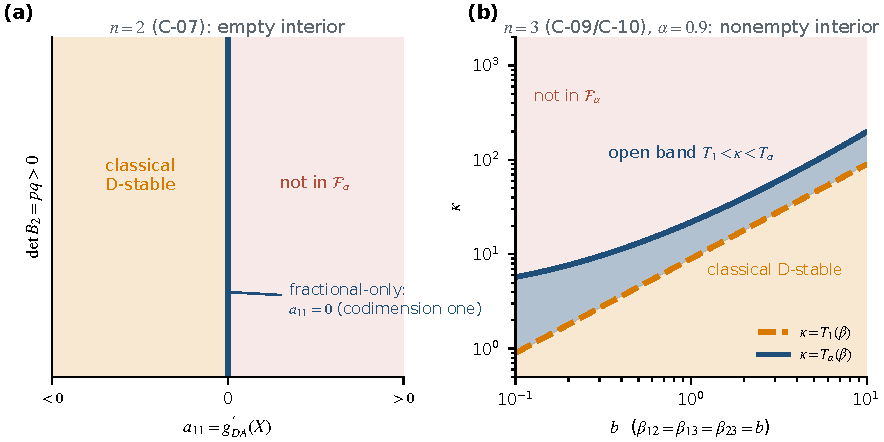
\includegraphics[width=0.90\textwidth]{fig02_dimension_contrast.pdf}
\caption{Dimension contrast. In two dimensions the genuinely fractional all-diagonal class is confined to a lower-dimensional equality set. In three dimensions the exact thresholds \(T_1(\beta)\) and \(T_\alpha(\beta)\) enclose an open fractional-only band. The three-dimensional panel anticipates Theorem~\ref{thm:c10}.}
\label{fig:dimcontrast}
\end{figure}

Theorem~\ref{thm:2d} is the lower-dimensional half of the minimum-dimension result. The remaining task is to show that dimension three contains full-dimensional open subsets of \(\mathcal P_\alpha^{(3)}\) for every \(0<\alpha<1\).

\section{Exact Dimension-Three Characterization}\label{sec:three}

We now specialize the simplex reduction to real \(3\times3\) matrices. Assume first that \(-A\) is a strict \(P\)-matrix and write
\[
p_i=-a_{ii}>0,\qquad
m_{12},m_{13},m_{23}>0,\qquad
q=-\det A>0,
\]
with the normalized invariants in Equation~\eqref{eq:four-invariants}. For
\[
D=\diag(d_1,d_2,d_3)\succ0
\]
the characteristic polynomial is
\begin{equation}
\det(\lambda I-DA)
=
\lambda^3+a_D\lambda^2+b_D\lambda+c_D,
\label{eq:cubicD}
\end{equation}
where
\begin{align}
a_D&=p_1d_1+p_2d_2+p_3d_3,\\
b_D&=m_{12}d_1d_2+m_{13}d_1d_3+m_{23}d_2d_3,\\
c_D&=q\,d_1d_2d_3.
\end{align}
With
\[
x_i=\frac{p_id_i}{a_D},
\qquad x\in\Delta_2^\circ,
\]
define
\begin{equation}
B_\beta(x)
=
\beta_{12}x_1x_2+
\beta_{13}x_1x_3+
\beta_{23}x_2x_3.
\label{eq:Bbeta}
\end{equation}
Then
\begin{equation}
\frac{b_D}{a_D^2}=B_\beta(x),
\qquad
\frac{c_D}{a_D^3}=\kappa x_1x_2x_3.
\label{eq:normalized-coeffs}
\end{equation}

\subsection{The Fixed-Cubic Matignon Boundary}

The fixed-polynomial component is a fractional Routh--Hurwitz/root-location problem; related coefficient-space criteria are established in the literature \cite{CermakNechvatal2017,BourafaAbdelouahabMoussaoui2020}. We state the exact form required for the diagonal-orbit elimination.

\begin{Lemma}[boundary value for a positive cubic]\label{lem:cubic-boundary}
Let
\[
p(\lambda)=\lambda^3+a\lambda^2+b\lambda+c,
\qquad a,b,c>0,
\]
and let
\[
\frac{\pi}{3}<\theta<\frac{\pi}{2}.
\]
Set
\[
u=\cos\theta,\qquad K=1-4u^2>0,
\]
and define
\begin{equation}
r_\theta(a,b)
=
\frac{ua+\sqrt{u^2a^2+Kb}}{K},
\qquad
H_\theta(a,b)
=
r_\theta(a,b)^2\bigl(a+2ur_\theta(a,b)\bigr).
\label{eq:Htheta}
\end{equation}
Then
\begin{equation}
|\arg\lambda_j|>\theta\quad\forall j
\quad\Longleftrightarrow\quad
c<H_\theta(a,b).
\label{eq:fixed-cubic-iff}
\end{equation}
Equality places one conjugate pair exactly on the rays \(|\arg\lambda|=\theta\). Moreover,
\[
H_\theta(sa,s^2b)=s^3H_\theta(a,b)
\qquad(s>0).
\]
\end{Lemma}

\begin{proof}
A polynomial with positive coefficients has no positive real zero, so loss of Matignon stability can occur only through a conjugate pair crossing a boundary ray. Put \(\lambda=re^{i\theta}\), \(r>0\), in \(p(\lambda)=0\). Dividing the imaginary part by \(r\sin\theta\) gives
\[
r^2\frac{\sin3\theta}{\sin\theta}
+
ar\frac{\sin2\theta}{\sin\theta}
+b=0.
\]
Using
\[
\frac{\sin3\theta}{\sin\theta}=4u^2-1=-K,
\qquad
\frac{\sin2\theta}{\sin\theta}=2u,
\]
we obtain
\[
Kr^2-2uar-b=0,
\]
whose unique positive solution is \(r=r_\theta(a,b)\). The real part then gives
\[
c=r^2(a+2ur)=H_\theta(a,b).
\]
For \(c>0\) sufficiently small, the roots consist of a small negative real root and a perturbation of the roots of \(\lambda^2+a\lambda+b\), hence are inside the Matignon region. For \(c\to\infty\), the roots approach the cube-root directions of \(-c\), including arguments \(\pm\pi/3\), which violate \(\theta>\pi/3\). Since there is only one boundary value, Equation~\eqref{eq:fixed-cubic-iff} follows. Homogeneity is immediate from Equation~\eqref{eq:Htheta}.
\end{proof}

For \(2/3<\alpha<1\), put \(\theta=\alpha\pi/2\) and define
\begin{equation}
h_\alpha(b):=H_\theta(1,b).
\end{equation}
Equivalently,
\begin{equation}
r_\alpha(b)
=
\frac{u+\sqrt{u^2+(1-4u^2)b}}{1-4u^2},
\qquad
h_\alpha(b)
=
r_\alpha(b)^2\bigl(1+2ur_\alpha(b)\bigr),
\label{eq:halpha}
\end{equation}
where \(u=\cos(\alpha\pi/2)\).

\subsection{Exact Elimination of the Positive-Diagonal Orbit}

Define
\begin{equation}
T_\alpha(\beta)
=
\min_{x\in\Delta_2^\circ}
\frac{h_\alpha(B_\beta(x))}{x_1x_2x_3}.
\label{eq:Talpha}
\end{equation}
The minimum is attained in the simplex interior because the numerator remains positive on the closed simplex while \(x_1x_2x_3\to0\) on its boundary.

\begin{Theorem}[exact three-dimensional Matignon \(D\)-stability]\label{thm:c10}
Let \(-A\) be a strict \(P\)-matrix and let \(2/3<\alpha<1\). Then
\begin{equation}
\boxed{
A\in\mathcal F_\alpha^{(3)}
\quad\Longleftrightarrow\quad
\kappa<T_\alpha(\beta).
}
\label{eq:c10-iff}
\end{equation}
\end{Theorem}

\begin{proof}
For a positive diagonal \(D\), let \(s=a_D\) and let \(x\in\Delta_2^\circ\) be its normalized orbit coordinate. Equations~\eqref{eq:normalized-coeffs} give
\[
a_D=s,\qquad
b_D=s^2B_\beta(x),\qquad
c_D=s^3\kappa x_1x_2x_3.
\]
By Lemma~\ref{lem:cubic-boundary} and homogeneity,
\[
\spec(DA)\subset\Sigma_\alpha
\]
is equivalent to
\[
\kappa
<
\frac{h_\alpha(B_\beta(x))}{x_1x_2x_3}.
\]
The normalization \(D\mapsto x\) is onto the open simplex modulo common scale. Hence the inequality must hold for every \(D\succ0\) if and only if it holds for every \(x\in\Delta_2^\circ\), which is exactly Equation~\eqref{eq:c10-iff}.
\end{proof}

The theorem is an explicit low-dimensional solution of a generalized multiplicative \(D\)-stability problem. Abstract forbidden-boundary criteria for conic regions and complements are already known \cite{KushelPavaniJDDE}; the step established in Theorem~\ref{thm:c10} is the complete elimination of the universal diagonal multiplier into the four invariants and the scalar threshold~\eqref{eq:Talpha}.

\subsection{Interior and the Classical Cain Boundary}

The strict-\(P\) hypothesis is exactly the full-dimensional stratum relevant to the interior.

\begin{Lemma}[principal-minor necessity]\label{lem:P0}
If \(A\in\mathcal F_\alpha^{(3)}\), then
\[
-a_{ii}\ge0,\qquad
\det A[\{i,j\}]\ge0,\qquad
-\det A>0.
\]
Consequently, every interior point of \(\mathcal F_\alpha^{(3)}\) has \(-A\) strict \(P\).
\end{Lemma}

\begin{proof}
If some \(a_{ii}>0\), let the other row scalings tend to zero; the limiting matrix has a positive real eigenvalue, and nearby positive diagonal scalings violate Matignon stability. If an order-two principal minor is negative, the same argument with the complementary row scaling tending to zero produces a \(2\times2\) block with a positive real eigenvalue. Finally a real \(3\times3\) Matignon-stable matrix has negative determinant, so \(-\det A>0\). Any zero order-one or order-two signed principal minor can be perturbed arbitrarily slightly to the forbidden sign, and therefore cannot occur at an interior point.
\end{proof}

At the classical endpoint \(\alpha=1\),
\[
h_1(b)=b,
\]
so
\begin{equation}
T_1(\beta)
=
\min_{x\in\Delta_2^\circ}
\left(
\frac{\beta_{23}}{x_1}
+
\frac{\beta_{13}}{x_2}
+
\frac{\beta_{12}}{x_3}
\right).
\end{equation}
Cauchy--Schwarz gives the exact value
\begin{equation}
\boxed{
T_1(\beta)
=
\left(
\sqrt{\beta_{12}}+
\sqrt{\beta_{13}}+
\sqrt{\beta_{23}}
\right)^2,
}
\label{eq:T1}
\end{equation}
which is Cain's strict-\(P\) real \(3\times3\) \(D\)-stability threshold \cite{Cain1976}.

For \(2/3<\alpha<1\), \(T_\alpha\) lies strictly above this classical surface. Indeed, from
\[
b=(1-4u^2)r^2-2ur
\]
and Equation~\eqref{eq:halpha},
\[
h_\alpha(b)-b
=
4u^2r^2+2ur(r^2+1)>0.
\]
Therefore
\begin{equation}
\boxed{
T_\alpha(\beta)>T_1(\beta)
\qquad(2/3<\alpha<1).
}
\label{eq:strict-gap}
\end{equation}

\begin{Corollary}[exact genuinely fractional band]\label{cor:fracband}
For \(2/3<\alpha<1\),
\begin{equation}
\operatorname{int}\mathcal P_\alpha^{(3)}
=
\left\{
A:
-A\text{ strict }P,\quad
T_1(\beta)<\kappa<T_\alpha(\beta)
\right\}.
\label{eq:fractional-band}
\end{equation}
For \(0<\alpha\le2/3\),
\begin{equation}
\operatorname{int}\mathcal F_\alpha^{(3)}
=
\{A:-A\text{ strict }P\},
\label{eq:low-order-F}
\end{equation}
and
\begin{equation}
\operatorname{int}\mathcal P_\alpha^{(3)}
=
\left\{
A:
-A\text{ strict }P,\quad
\kappa>T_1(\beta)
\right\}.
\label{eq:low-order-P}
\end{equation}
\end{Corollary}

\begin{proof}
The high-order statement follows from Theorem~\ref{thm:c10}, Equation~\eqref{eq:T1}, and strictness of the inequalities. In the low-order regime, Kellogg's eigenvalue wedge theorem for \(P\)-matrices \cite{Kellogg1972} implies that if \(-A\) is strict \(P\), every eigenvalue of \(-DA\) lies in
\[
|\arg\mu|<\pi-\frac{\pi}{3}=\frac{2\pi}{3}.
\]
After multiplication by \(-1\), the eigenvalues of \(DA\) satisfy the Matignon inequality for every \(\alpha\le2/3\). Lemma~\ref{lem:P0} gives necessity for interior points, while Cain's threshold separates classical \(D\)-stability from its complement.
\end{proof}

Figure~\ref{fig:c10geometry} shows the exact threshold geometry on symmetric and asymmetric slices. The blue Matignon boundary remains strictly above the orange Cain boundary, and the region between them is precisely the all-positive-diagonal fractional-only band.

\begin{figure}[!htbp]
\centering
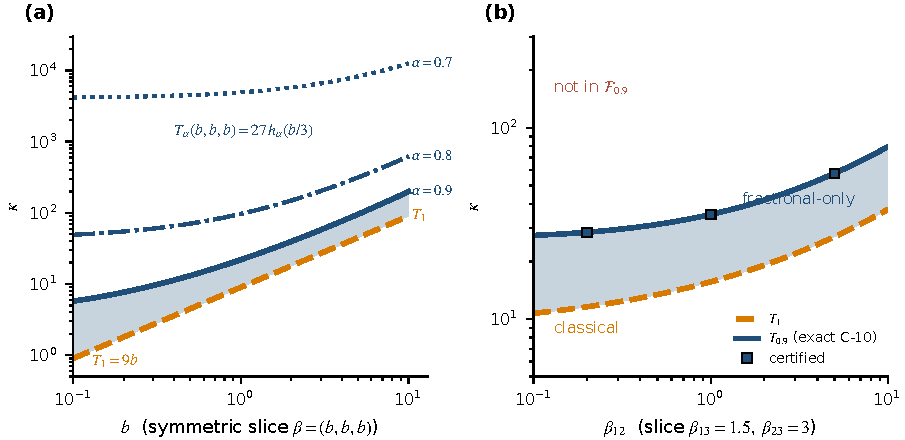
\includegraphics[width=0.92\textwidth]{fig03_threshold_geometry.pdf}
\caption{Exact C-10 threshold geometry. The orange curve is Cain's classical boundary \(T_1(\beta)\); the blue curve is the exact Matignon boundary \(T_\alpha(\beta)\). Their strict separation creates the genuinely fractional band. Certified anchor markers are computational checks of exact formulas, not substitutes for Theorem~\ref{thm:c10}.}
\label{fig:c10geometry}
\end{figure}

\subsection{Minimum Dimension for a Robust Fractional-Only Class}

The two-dimensional obstruction and the three-dimensional band give the dimension result.

\begin{Theorem}[minimum robust dimension]\label{thm:mindim}
For every \(0<\alpha<1\),
\begin{equation}
\boxed{
\min\left\{
n:
\operatorname{int}
\left(
\mathcal F_\alpha^{(n)}
\setminus
\mathcal D_H^{(n)}
\right)\ne\varnothing
\right\}=3.
}
\label{eq:min-dim}
\end{equation}
\end{Theorem}

\begin{proof}
Dimension one is trivial and Theorem~\ref{thm:2d} gives empty full-dimensional interior in dimension two. For \(2/3<\alpha<1\), Equation~\eqref{eq:strict-gap} makes the interval
\[
T_1(\beta)<\kappa<T_\alpha(\beta)
\]
nonempty for every positive \(\beta\); any strict interior point is stable under small full-matrix perturbations. For \(0<\alpha\le2/3\), choose any strict-\(P(-A)\) matrix violating Cain's inequality \(\kappa<T_1(\beta)\). Corollary~\ref{cor:fracband} then places it in \(\mathcal P_\alpha^{(3)}\), and strictness again gives a full-dimensional neighborhood.
\end{proof}

\section{Geometry and Order Dependence of the Exact Threshold}\label{sec:geometry}

The exact criterion in Theorem~\ref{thm:c10} reduces the complete positive-diagonal orbit to the scalar threshold \(T_\alpha(\beta)\). We next show that this variational quantity has substantially more structure than a generic two-variable minimum.

\subsection{Strict Convexity and a Unique Optimizer}

Fix \(2/3<\alpha<1\). Let
\[
 u=\cos\!\left(\frac{\alpha\pi}{2}\right),\qquad
 K_\alpha=1-4u^2,
\]
and recall from Equation~\eqref{eq:halpha} that \(h_\alpha(b)=r^2(1+2ur)\), where \(r\) is the positive solution of
\[
 b=K_\alpha r^2-2ur.
\]
Introduce the elasticity
\begin{equation}
 E_\alpha(b)
 :=
 \frac{b\,h_\alpha'(b)}{h_\alpha(b)}.
 \label{eq:elasticity}
\end{equation}

\begin{Lemma}[elasticity bounds]\label{lem:elasticity}
For every \(b>0\),
\begin{equation}
 0<E_\alpha(b)<\frac32,
 \qquad
 \frac{dE_\alpha}{db}>0.
 \label{eq:elasticity-bounds}
\end{equation}
\end{Lemma}

\begin{proof}
Using \(r\) as parameter,
\[
 \frac{db}{dr}=2(K_\alpha r-u),
 \qquad
 \frac{dh_\alpha}{dr}=2r(1+3ur),
\]
and therefore
\begin{equation}
 E_\alpha
 =
 \frac{(K_\alpha r-2u)(1+3ur)}
      {(K_\alpha r-u)(1+2ur)}.
 \label{eq:E-r}
\end{equation}
On \(r>2u/K_\alpha\), both factors
\[
 \frac{K_\alpha r-2u}{K_\alpha r-u},
 \qquad
 \frac{1+3ur}{1+2ur}
\]
increase strictly with \(r\). Their product increases from \(0\) to \(3/2\). Since \(b(r)\) is strictly increasing, Equation~\eqref{eq:elasticity-bounds} follows.
\end{proof}

Parameterize the open simplex by logit variables
\begin{equation}
 x_1=\frac{e^{y_1}}{e^{y_1}+e^{y_2}+1},
 \quad
 x_2=\frac{e^{y_2}}{e^{y_1}+e^{y_2}+1},
 \quad
 x_3=\frac{1}{e^{y_1}+e^{y_2}+1}.
 \label{eq:logit}
\end{equation}
Set
\[
 L(y)=\log(e^{y_1}+e^{y_2}+1),
\]
\[
 Q_\beta(y)
 =
 \log\!\left(
 \beta_{12}e^{y_1+y_2}
 +\beta_{13}e^{y_1}
 +\beta_{23}e^{y_2}
 \right),
\]
and \(\phi_\alpha(s)=\log h_\alpha(e^s)\). Then
\begin{equation}
 G_{\alpha,\beta}(y)
 :=
 \log\!\left[
 \frac{h_\alpha(B_\beta(x(y)))}{x_1x_2x_3}
 \right]
 =
 \phi_\alpha(Q_\beta-2L)+3L-y_1-y_2.
 \label{eq:logobjective}
\end{equation}

\begin{Theorem}[strict threshold geometry]\label{thm:strict-convexity}
For every \(\beta\in\mathbb R_{>0}^3\) and \(2/3<\alpha<1\), \(G_{\alpha,\beta}\) is globally strictly convex on \(\mathbb R^2\). Hence:
\begin{enumerate}
\item \(T_\alpha(\beta)\) has a unique minimizer \(x^*(\alpha,\beta)\in\Delta_2^\circ\);
\item the minimizer is nondegenerate;
\item \(x^*\) and \(T_\alpha\) depend smoothly on \((\alpha,\beta)\).
\end{enumerate}
\end{Theorem}

\begin{proof}
Put \(s=Q_\beta-2L\). Since
\[
 \phi_\alpha'(\log b)=E_\alpha(b),
 \qquad
 \phi_\alpha''(\log b)=b\,E_\alpha'(b),
\]
Lemma~\ref{lem:elasticity} gives
\[
 \phi_\alpha'>0,\qquad
 \phi_\alpha''>0,\qquad
 3-2\phi_\alpha'>0.
\]
Differentiating Equation~\eqref{eq:logobjective},
\begin{equation}
 \nabla^2G_{\alpha,\beta}
 =
 \phi_\alpha''\,\nabla s\nabla s^\top
 +\phi_\alpha'\nabla^2Q_\beta
 +(3-2\phi_\alpha')\nabla^2L.
 \label{eq:hessian-decomp}
\end{equation}
Both \(Q_\beta\) and \(L\) are log-sum-exp functions of affine forms, so \(\nabla^2Q_\beta\succeq0\); moreover \(\nabla^2L\succ0\) because all three softmax weights are positive. Every coefficient in Equation~\eqref{eq:hessian-decomp} is nonnegative and the coefficient of \(\nabla^2L\) is strictly positive. Thus \(\nabla^2G_{\alpha,\beta}\succ0\) everywhere.

As \(\|y\|\to\infty\), \(x(y)\) approaches the simplex boundary and \(x_1x_2x_3\to0\), while \(h_\alpha(B_\beta(x))\) remains positive. Hence \(G_{\alpha,\beta}\) is coercive. A unique minimizer exists; positive definiteness gives nondegeneracy, and the implicit-function theorem gives smooth dependence.
\end{proof}

Two exact reductions follow immediately. If \(\beta_{12}=\beta_{13}=\beta_{23}=b\), uniqueness and permutation symmetry imply \(x^*=(1/3,1/3,1/3)\), so
\begin{equation}
 T_\alpha(b,b,b)=27h_\alpha(b/3).
 \label{eq:symmetric-slice}
\end{equation}
For \(b=1\), this becomes the cyclic-network boundary
\begin{equation}
 T_\alpha(1,1,1)=1+R_3(\alpha)^3,
 \qquad
 R_3(\alpha)
 =
 \frac{\sin(\alpha\pi/2)}
 {\sin(\alpha\pi/2-\pi/3)},
 \label{eq:siami-slice}
\end{equation}
recovering the structured slice studied by Siami \cite{Siami2021}. If two \(\beta\)'s are equal, the corresponding two simplex coordinates of \(x^*\) are equal, reducing the minimization exactly to one dimension.

\subsection{Dependence on the Fractional Order}

\begin{Theorem}[monotone widening and the classical limit]\label{thm:alpha-deformation}
For fixed \(\beta>0\), \(T_\alpha(\beta)\) is strictly decreasing in \(\alpha\) on \(2/3<\alpha\le1\). Let
\[
 S=\sqrt{\beta_{12}}+\sqrt{\beta_{13}}+\sqrt{\beta_{23}},
 \qquad
 G=\sqrt{\beta_{12}\beta_{13}\beta_{23}}.
\]
As \(\alpha\to1^{-}\),
\begin{equation}
 T_\alpha(\beta)
 =
 T_1(\beta)
 +
 C(\beta)(1-\alpha)
 +
 O((1-\alpha)^2),
 \label{eq:classical-rate}
\end{equation}
where
\begin{equation}
 C(\beta)
 =
 \pi\left(
 \frac{S^{5/2}}{\sqrt G}
 +
 S^{3/2}\sqrt G
 \right)>0.
 \label{eq:Cbeta}
\end{equation}
\end{Theorem}

\begin{proof}
For fixed positive \(a,b\), decreasing the boundary angle \(\theta=\alpha\pi/2\) strictly enlarges the Matignon region. The unique coefficient value \(H_\theta(a,b)\) placing a conjugate pair on the boundary therefore increases strictly as \(\theta\) decreases. Hence \(h_{\alpha_1}(b)>h_{\alpha_2}(b)\) whenever \(\alpha_1<\alpha_2\), and minimization over the same simplex preserves strictness.

For the rate, \(u=\cos(\alpha\pi/2)=\frac{\pi}{2}(1-\alpha)+O((1-\alpha)^3)\). Implicit differentiation of
\[
 (1-4u^2)r^2-2ur-b=0
\]
at \(u=0\) gives \(\partial r/\partial u=1\). Consequently
\begin{equation}
 h_\alpha(b)
 =
 b+\pi(1-\alpha)\sqrt b(1+b)+O((1-\alpha)^2).
 \label{eq:h-expansion}
\end{equation}
At \(\alpha=1\), the unique simplex minimizer is
\[
 x_1^*=\frac{\sqrt{\beta_{23}}}{S},
 \quad
 x_2^*=\frac{\sqrt{\beta_{13}}}{S},
 \quad
 x_3^*=\frac{\sqrt{\beta_{12}}}{S},
\]
for which
\[
 x_1^*x_2^*x_3^*=\frac{G}{S^3},
 \qquad
 B_\beta(x^*)=\frac{G}{S}.
\]
The envelope theorem applied to the nondegenerate minimum and Equation~\eqref{eq:h-expansion} yields Equations~\eqref{eq:classical-rate}--\eqref{eq:Cbeta}.
\end{proof}

Theorem~\ref{thm:alpha-deformation} quantifies the part of the order dependence that is needed below: the fractional-only band widens strictly as \(\alpha\) decreases and closes linearly at the classical endpoint. Together with the exact symmetric reductions above, this supplies a smooth and uniquely optimized threshold geometry without adding further parameters to the C-10 classification.

\section{A Nonlinear Caputo Double-Allee Ecological Realization}\label{sec:ecology}

We now ask whether the open matrix band in Equation~\eqref{eq:fractional-band} can be realized by a biologically standard nonlinear Kolmogorov system rather than by an abstract matrix construction. The answer depends on the interaction architecture. The first natural model fails for a structural reason; an intraguild-predation architecture removes precisely that obstruction.

\subsection{Positive-Equilibrium Orbit Equivalence}

Consider a commensurate Caputo Kolmogorov system
\begin{equation}
 {}^C D_t^\alpha x_i=x_iF_i(x),\qquad i=1,\dots,n,
 \label{eq:kolmogorov-general}
\end{equation}
and let \(x^*\gg0\) be an equilibrium. Put \(B=DF(x^*)\).

\begin{Lemma}[Kolmogorov orbit equivalence]\label{lem:kolmogorov-orbit}
At a positive equilibrium,
\begin{equation}
 J(x^*)=\diag(x^*)B.
 \label{eq:kolmogorov-jacobian}
\end{equation}
Consequently,
\[
 J(x^*)\in\mathcal F_\alpha^{(n)}
 \iff
 B\in\mathcal F_\alpha^{(n)},
 \qquad
 J(x^*)\in\mathcal D_H^{(n)}
 \iff
 B\in\mathcal D_H^{(n)}.
\]
\end{Lemma}

\begin{proof}
For \(G_i(x)=x_iF_i(x)\),
\[
 \partial_jG_i
 =
 \delta_{ij}F_i+x_i\partial_jF_i.
\]
At \(x^*\), \(F_i(x^*)=0\), which gives Equation~\eqref{eq:kolmogorov-jacobian}. Since \(D\mapsto D\diag(x^*)\) is a bijection of the positive diagonal cone onto itself, the two positive-diagonal spectral orbits coincide.
\end{proof}

This factorization is standard in Kolmogorov-system stability theory and is used here only as a bridge \cite{HouBaigent2015,ChenWangLiu2024}.

\subsection{A Structural No-Go for Two Competing Consumers}

Begin with a double-Allee basal prey consumed by two competitors:
\begin{align}
 {}^CD_t^\alpha x&=x[g_{\rm DA}(x)-q_1y-q_2z],\nonumber\\
 {}^CD_t^\alpha y&=y[e_1q_1x-\mu_1-c_{11}y-c_{12}z],\label{eq:competitive-model}\\
 {}^CD_t^\alpha z&=z[e_2q_2x-\mu_2-c_{21}y-c_{22}z],\nonumber
\end{align}
with positive parameters. At a positive equilibrium let \(s=-g_{\rm DA}'(X)>0\). The reduced matrix is
\begin{equation}
 B_{\rm comp}
 =
 \begin{pmatrix}
 -s&-q_1&-q_2\\
 e_1q_1&-c_{11}&-c_{12}\\
 e_2q_2&-c_{21}&-c_{22}
 \end{pmatrix}.
 \label{eq:Bcomp}
\end{equation}
On its strict-\(P\) stratum,
\begin{align}
 \beta_{12}&=1+\frac{e_1q_1^2}{sc_{11}},&
 \beta_{13}&=1+\frac{e_2q_2^2}{sc_{22}},&
 \beta_{23}&=1-\frac{c_{12}c_{21}}{c_{11}c_{22}}>0,
 \label{eq:competitive-betas}
\end{align}
and the normalized directed three-cycle contribution is
\begin{equation}
 L_3
 =
 \frac{q_1q_2(c_{12}e_2+c_{21}e_1)}
 {sc_{11}c_{22}}>0.
 \label{eq:competitive-L3}
\end{equation}
The determinant identity
\begin{equation}
 \kappa
 =
 \beta_{12}+\beta_{13}+\beta_{23}-2-L_3
 \label{eq:kappa-loop}
\end{equation}
then yields the following obstruction.

\begin{Theorem}[competitive-architecture no-go]\label{thm:no-go}
Every strict-\(P\) point of the model in Equation~\eqref{eq:competitive-model} is classically Hurwitz \(D\)-stable. In particular, the architecture cannot realize an open set satisfying
\[
 T_1(\beta)<\kappa<T_\alpha(\beta).
\]
\end{Theorem}

\begin{proof}
From Equations~\eqref{eq:competitive-L3}--\eqref{eq:kappa-loop},
\[
 \kappa
 <
 \beta_{12}+\beta_{13}+\beta_{23}-2
 <
 \beta_{12}+\beta_{13}+\beta_{23}.
\]
Because all \(\beta_{ij}>0\),
\[
 T_1(\beta)
 =
 \left(
 \sqrt{\beta_{12}}+\sqrt{\beta_{13}}+\sqrt{\beta_{23}}
 \right)^2
 >
 \beta_{12}+\beta_{13}+\beta_{23}.
\]
Thus \(\kappa<T_1(\beta)\), which is exactly Cain's strict-\(P\) \(D\)-stability inequality.
\end{proof}

The failure is therefore architectural rather than parametric: adding more parameter search cannot reverse the sign in Equation~\eqref{eq:competitive-L3}.

\subsection{Intraguild Predation and Exact Invariant Access}

We replace direct competition between the consumers by intraguild predation/omnivory, a standard three-species motif \cite{HoltPolis1997,BaiKangRuanWang2021,Panja2019}:
\begin{align}
 {}^CD_t^\alpha x
 &=
 x[g_{\rm DA}(x)-q_1y-q_2z],
 \nonumber\\
 {}^CD_t^\alpha y
 &=
 y[e_1q_1x-\mu_1-c_1y-hz],
 \label{eq:igp-model}\\
 {}^CD_t^\alpha z
 &=
 z[e_2q_2x+e_3hy-\mu_2-c_2z],
 \nonumber
\end{align}
where
\begin{equation}
 g_{\rm DA}(x)
 =
 \frac{r}{x+a}
 \left(1-\frac{x}{K}\right)(x-m),
 \qquad
 0<m<K,
 \label{eq:gDA}
\end{equation}
and all displayed parameters are positive. Here \(x\) is the basal prey/resource, \(y\) the intermediate consumer or intraguild prey, and \(z\) the omnivorous top predator.

At a positive equilibrium \((X,Y,Z)\),
\begin{align}
 g_{\rm DA}(X)&=q_1Y+q_2Z,\label{eq:eq1}\\
 c_1Y+hZ&=e_1q_1X-\mu_1,\label{eq:eq2}\\
 -e_3hY+c_2Z&=e_2q_2X-\mu_2.\label{eq:eq3}
\end{align}
Put
\[
 \Delta=c_1c_2+e_3h^2,
 \quad
 A_1=e_1q_1X-\mu_1,
 \quad
 A_2=e_2q_2X-\mu_2.
\]
Then
\begin{equation}
 Y=\frac{c_2A_1-hA_2}{\Delta},
 \qquad
 Z=\frac{e_3hA_1+c_1A_2}{\Delta}.
 \label{eq:YZ}
\end{equation}
Moreover
\begin{equation}
 q_1Y+q_2Z=\chi X-\nu,
 \label{eq:affine-predation}
\end{equation}
where
\begin{equation}
 \chi=
 \frac{
 e_1c_2q_1^2+e_2c_1q_2^2
 +hq_1q_2(e_1e_3-e_2)
 }{\Delta},
 \label{eq:chi}
\end{equation}
and
\[
 \nu=
 \frac{
 \mu_1(q_1c_2+q_2e_3h)
 +\mu_2(q_2c_1-q_1h)
 }{\Delta}.
\]
Thus \(X\) satisfies the degree-at-most-two equation
\begin{equation}
 (r+K\chi)X^2
 -
 [r(K+m)-K\chi a+K\nu]X
 +
 rKm-K\nu a
 =0.
 \label{eq:Xquadratic}
\end{equation}
In the constructive regime used below \(e_1e_3\ge e_2\), so \(\chi>0\) and Equation~\eqref{eq:Xquadratic} is a genuine quadratic.

At coexistence set
\[
 s=-g_{\rm DA}'(X).
\]
The reduced per-capita matrix is
\begin{equation}
 B=
 \begin{pmatrix}
 -s&-q_1&-q_2\\
 e_1q_1&-c_1&-h\\
 e_2q_2&e_3h&-c_2
 \end{pmatrix}.
 \label{eq:Bigp}
\end{equation}
Its order-two principal minors are
\[
 m_{12}=sc_1+e_1q_1^2,\quad
 m_{13}=sc_2+e_2q_2^2,\quad
 m_{23}=c_1c_2+e_3h^2,
\]
and a direct determinant calculation gives
\begin{equation}
 -\det B
 =
 \Delta(s+\chi).
 \label{eq:q-delta}
\end{equation}
Hence the exact strict-\(P\) condition for this architecture is
\begin{equation}
 s>0,\qquad s+\chi>0.
 \label{eq:igp-strictP}
\end{equation}
The four C-10 invariants are
\begin{align}
 \beta_{12}&=1+\frac{e_1q_1^2}{sc_1},&
 \beta_{13}&=1+\frac{e_2q_2^2}{sc_2},&
 \beta_{23}&=1+\frac{e_3h^2}{c_1c_2},
 \label{eq:igp-betas}\\
 \kappa
 &=
 \beta_{12}+\beta_{13}+\beta_{23}-2
 +
 \frac{hq_1q_2(e_1e_3-e_2)}{sc_1c_2}.
 \label{eq:igp-kappa}
\end{align}
Equivalently,
\begin{equation}
 L_3
 =
 \frac{hq_1q_2(e_2-e_1e_3)}{sc_1c_2}.
 \label{eq:igp-L3}
\end{equation}
Thus \(e_1e_3>e_2\) makes \(L_3<0\), the sign mechanism missing from the competitive architecture.

Figure~\ref{fig:mechanism} displays the two motifs and the corresponding directed-cycle sign. The diagram is a theorem schematic; no numerical data enter the no-go or realization argument.

\begin{figure}[H]
\centering
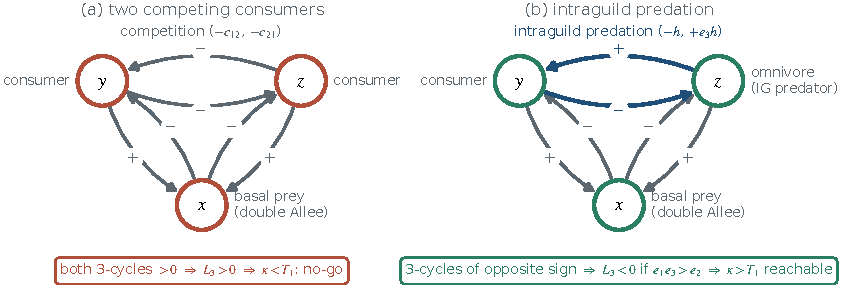
\includegraphics[width=0.94\textwidth]{fig05_ecological_mechanism.pdf}
\caption{Ecological architectures and the signed three-cycle mechanism. \textbf{(a)} With two competing consumers, both oriented three-cycles contribute with the sign that makes \(L_3>0\), forcing \(\kappa<T_1\) on the strict-\(P\) stratum. \textbf{(b)} Intraguild predation reverses one cycle; when \(e_1e_3>e_2\), \(L_3<0\) and access to \(\kappa>T_1\) becomes possible.}
\label{fig:mechanism}
\end{figure}

\begin{Theorem}[four-invariant IGP realization]\label{thm:igp-realization}
Fix
\[
 \beta_{12},\beta_{13},\beta_{23}>1
\]
and
\begin{equation}
 \kappa>
 \beta_{12}+\beta_{13}+\beta_{23}-2.
 \label{eq:igp-target}
\end{equation}
Then positive IGP parameters can be chosen so that the matrix in Equation~\eqref{eq:Bigp} has exactly these four invariants. The construction may be made with
\[
 0<e_1,e_2,e_3<1,
 \qquad
 e_1e_3>e_2.
\]
\end{Theorem}

\begin{proof}
Let
\[
 A=\beta_{12}-1,\quad
 B_0=\beta_{13}-1,\quad
 C=\beta_{23}-1,
\]
and
\[
 R=\kappa-(\beta_{12}+\beta_{13}+\beta_{23}-2)>0.
\]
Put
\[
 \rho=\frac{R}{\sqrt{AB_0C}},
 \qquad
 \tau=\frac{\rho+\sqrt{\rho^2+4}}{2}>1,
\]
so \(\tau-\tau^{-1}=\rho\). Choose any \(\eta\in(0,1)\) and set
\[
 e_1=e_3=\eta,
 \qquad
 e_2=\frac{\eta^2}{\tau^2}.
\]
For arbitrary \(s,c_1,c_2>0\), define
\begin{equation}
 q_1=\sqrt{\frac{Asc_1}{e_1}},
 \qquad
 q_2=\sqrt{\frac{B_0sc_2}{e_2}},
 \qquad
 h=\sqrt{\frac{Cc_1c_2}{e_3}}.
 \label{eq:igp-right-inverse}
\end{equation}
Equations~\eqref{eq:igp-betas} give the prescribed \(\beta\)'s, while
\[
 \frac{hq_1q_2(e_1e_3-e_2)}{sc_1c_2}
 =
 \sqrt{AB_0C}\left(\tau-\frac1\tau\right)
 =R.
\]
Equation~\eqref{eq:igp-kappa} then gives the prescribed \(\kappa\). Since \(\tau>1\), \(e_1e_3>e_2\).
\end{proof}

\subsection{Embedding the Invariants in the Double-Allee Model}

The previous theorem fixes the desired local prey self-slope \(s>0\). We now realize it at a positive equilibrium of Equation~\eqref{eq:igp-model}.

Fix
\[
 a>0,\qquad 0<m<X<K,
\]
and define
\begin{equation}
 H_A
 =
 \frac{1}{K-X}
 -
 \frac{1}{X-m}
 +
 \frac{1}{X+a}.
 \label{eq:HA}
\end{equation}
Writing
\[
 C_A=\frac{m+a}{(X-m)(X+a)},
\]
we have \(H_A=(K-X)^{-1}-C_A\), so \(H_A>0\) precisely when
\begin{equation}
 X<K<
 K_{\max}
 :=
 X+\frac{(X-m)(X+a)}{m+a}.
 \label{eq:Kmax}
\end{equation}
Set
\[
 Q=\frac{s}{H_A}.
\]
Choose \(\xi\in(0,1)\) and prescribe
\begin{equation}
 Y=\frac{\xi Q}{q_1},
 \qquad
 Z=\frac{(1-\xi)Q}{q_2}.
 \label{eq:YZsplit}
\end{equation}
Then \(q_1Y+q_2Z=Q\). Define
\begin{align}
 \mu_1&=e_1q_1X-c_1Y-hZ,\label{eq:mu1}\\
 \mu_2&=e_2q_2X+e_3hY-c_2Z.\label{eq:mu2}
\end{align}
The first mortality is positive whenever
\[
 Q<Q_1:=
 \frac{e_1q_1X}
 {\xi c_1/q_1+(1-\xi)h/q_2}.
\]
If \((1-\xi)c_2/q_2-\xi e_3h/q_1>0\), the second is positive whenever
\[
 Q<Q_2:=
 \frac{e_2q_2X}
 {(1-\xi)c_2/q_2-\xi e_3h/q_1};
\]
otherwise \(\mu_2>0\) automatically. Let \(\bar Q=Q_1\) in the latter case and \(\bar Q=\min(Q_1,Q_2)\) in the former. It is enough to choose
\begin{equation}
 0<K-X<
 \frac{1}{C_A+s/\bar Q}.
 \label{eq:K-close-bound}
\end{equation}
Finally set
\begin{equation}
 r=
 \frac{Q(X+a)}
 {(1-X/K)(X-m)}.
 \label{eq:r-embedding}
\end{equation}
Then \(g_{\rm DA}(X)=Q=q_1Y+q_2Z\), while
\[
 g_{\rm DA}'(X)
 =
 Q\left[
 -\frac1{K-X}
 +\frac1{X-m}
 -\frac1{X+a}
 \right]
 =-QH_A=-s.
\]
Thus the positive equilibrium has exactly the reduced matrix constructed in Theorem~\ref{thm:igp-realization}.

\begin{Theorem}[open genuinely fractional biological region]\label{thm:open-ecological}
For every fixed \(0<\alpha<1\), there exists a nonempty open set in the full positive biological parameter space of Equation~\eqref{eq:igp-model} for which a positive coexistence equilibrium on the constructed smooth branch satisfies
\begin{equation}
 J\in
 \mathcal F_\alpha^{(3)}
 \setminus
 \mathcal D_H^{(3)}.
 \label{eq:open-ecological-band}
\end{equation}
\end{Theorem}

\begin{proof}
If \(2/3<\alpha<1\), choose \(\beta\in(1,\infty)^3\) and
\[
 T_1(\beta)<\kappa<T_\alpha(\beta).
\]
Theorem~\ref{thm:igp-realization} gives an IGP reduced matrix with these invariants, and Equations~\eqref{eq:HA}--\eqref{eq:r-embedding} embed it at a positive double-Allee coexistence equilibrium. Theorem~\ref{thm:c10} gives \(B\in\mathcal F_\alpha^{(3)}\setminus\mathcal D_H^{(3)}\), and Lemma~\ref{lem:kolmogorov-orbit} transfers the statement to the actual Jacobian \(J\).

If \(0<\alpha\le2/3\), choose \(\beta>1\) and any \(\kappa>T_1(\beta)\) satisfying Equation~\eqref{eq:igp-target}. The construction is strict-\(P\), so Kellogg's wedge implies \(B\in\mathcal F_\alpha^{(3)}\), while Cain's inequality fails.

All feasibility and stability inequalities are strict. Moreover
\[
 -\det B=\kappa sc_1c_2>0,
\]
so the state Jacobian of the coexistence equations is nonsingular. The implicit-function theorem preserves the positive equilibrium on a smooth local branch under sufficiently small perturbations of all biological parameters, and continuity preserves the strict invariant inequalities. Hence the set is open in the full biological parameter space.
\end{proof}

\subsection{The Allee Threshold as a Monotone Invariant-Space Control}

After eliminating \(Y\) and \(Z\), the coexistence equation is
\begin{equation}
 F(X,m)
 :=
 g_{\rm DA}(X;m)-\chi X+\nu=0.
 \label{eq:scalar-equilibrium}
\end{equation}
Along a positive strict-\(P\) branch put
\[
 Q=g_{\rm DA}(X)=\chi X-\nu>0,
 \qquad
 s=-g_{\rm DA}'(X)>0.
\]
By Equation~\eqref{eq:q-delta},
\[
 s+\chi>0.
\]
Implicit differentiation gives the first exact monotonicity law:
\begin{equation}
 \frac{dX}{dm}
 =
 -\frac{Q}{(X-m)(s+\chi)}
 <0.
 \label{eq:dXdm}
\end{equation}

The slope \(s\) decreases as well. Set
\[
 d=X-m,\qquad
 \ell=K-X,\qquad
 w=X+a.
\]
Then \(H_A=\ell^{-1}-d^{-1}+w^{-1}\), and direct algebra gives
\begin{equation}
 \partial_XH_A-H_A^2
 =
 \frac{2(w-d)(\ell+w)}{d\ell w^2}>0,
 \label{eq:H-identity}
\end{equation}
because \(w-d=m+a>0\). Differentiating \(s=QH_A\) along Equation~\eqref{eq:scalar-equilibrium} yields
\begin{equation}
 \frac{ds}{dm}
 =
 -\frac{Q}{d(s+\chi)}
 \left[
 Q\partial_XH_A+\frac{s}{d}
 +\chi\left(H_A+\frac1d\right)
 \right].
 \label{eq:dsdm}
\end{equation}
Since strict-\(P\) gives \(\chi>-s\), the bracket is strictly larger than
\[
 Q\partial_XH_A+\frac{s}{d}
 -s\left(H_A+\frac1d\right)
 =
 Q(\partial_XH_A-H_A^2)>0.
\]
Therefore
\begin{equation}
 \boxed{
 \frac{dX}{dm}<0,\qquad
 \frac{ds}{dm}<0
 }
 \label{eq:allee-monotonicity}
\end{equation}
throughout the positive strict-\(P\) coexistence stratum. No sign assumption on \(\chi\) is required.

Put \(t=1/s\) and define
\[
 A_0=\frac{e_1q_1^2}{c_1},\quad
 B_0=\frac{e_2q_2^2}{c_2},\quad
 C_0=1+\frac{e_3h^2}{c_1c_2},\quad
 E_0=\frac{hq_1q_2(e_1e_3-e_2)}{c_1c_2}.
\]
Then
\begin{equation}
 \beta_{12}=1+A_0t,\quad
 \beta_{13}=1+B_0t,\quad
 \beta_{23}=C_0,\quad
 \kappa=C_0+(A_0+B_0+E_0)t,
 \label{eq:t-path}
\end{equation}
and Equation~\eqref{eq:allee-monotonicity} implies \(dt/dm>0\).

Along this path the classical gap is
\begin{align}
 G_1(t)
 &:=
 \kappa(t)-T_1(\beta(t))
 \nonumber\\
 &=
 E_0t-2
 -2\sqrt{(1+A_0t)(1+B_0t)}
 \nonumber\\
 &\quad
 -2\sqrt{C_0}
 \left[
 \sqrt{1+A_0t}
 +
 \sqrt{1+B_0t}
 \right].
 \label{eq:G1}
\end{align}

\begin{Theorem}[unique transverse Cain crossing]\label{thm:crossing}
If
\begin{equation}
 E_0>2\sqrt{A_0B_0},
 \label{eq:cross-condition}
\end{equation}
then \(G_1\) has a unique positive zero \(t_H\). The crossing is transverse and satisfies
\begin{equation}
 G_1'(t_H)
 \ge
 \frac{4+4\sqrt{C_0}}{t_H}
 >0.
 \label{eq:transversality}
\end{equation}
Consequently, because \(t\) increases strictly with \(m\), the coexistence branch crosses the classical \(D\)-stability boundary at most once and does so transversally.
\end{Theorem}

\begin{proof}
We have
\[
 G_1(0)=-4-4\sqrt{C_0}<0,
\]
whereas Equation~\eqref{eq:cross-condition} makes the asymptotic linear coefficient positive, so \(G_1(t)\to+\infty\). Direct differentiation shows
\begin{align}
 G_1''(t)
 &=
 \frac{(A_0-B_0)^2}
 {2[(1+A_0t)(1+B_0t)]^{3/2}}
 \nonumber\\
 &\quad+
 \sqrt{C_0}\left[
 \frac{A_0^2}{2(1+A_0t)^{3/2}}
 +
 \frac{B_0^2}{2(1+B_0t)^{3/2}}
 \right]>0.
\end{align}
Thus \(G_1\) is strictly convex and has exactly one positive root. Convexity gives
\[
 G_1'(t_H)
 \ge
 \frac{G_1(t_H)-G_1(0)}{t_H},
\]
which is Equation~\eqref{eq:transversality}.
\end{proof}

The crossing can be prescribed. For any \(t_0>0\), set
\begin{equation}
 E_0
 =
 \frac{
 2+2\sqrt{(1+A_0t_0)(1+B_0t_0)}
 +2\sqrt{C_0}\left[
 \sqrt{1+A_0t_0}+\sqrt{1+B_0t_0}
 \right]
 }{t_0}.
 \label{eq:prescribed-E0}
\end{equation}
Then \(G_1(t_0)=0\) and Equation~\eqref{eq:cross-condition} holds. Theorem~\ref{thm:igp-realization} realizes this \(E_0\) through a joint parameter choice, and the double-Allee embedding independently sets \(s_0=1/t_0\) at a selected \(m_0\). Hence, with every non-\(m\) model parameter fixed, there exists \(\varepsilon>0\) such that
\[
 m_0-\varepsilon<m<m_0
 \quad\Longrightarrow\quad
 J\in\mathcal D_H^{(3)},
\]
whereas
\begin{equation}
 m_0<m<m_0+\varepsilon
 \quad\Longrightarrow\quad
 J\in
 \mathcal F_\alpha^{(3)}
 \setminus
 \mathcal D_H^{(3)}.
 \label{eq:m-transition}
\end{equation}
For \(\alpha>2/3\), the right-hand implication follows from \(T_\alpha>T_1\) and continuity; for \(\alpha\le2/3\), strict-\(P\) itself gives fractional \(D\)-stability.

Figure~\ref{fig:m-path} visualizes this mechanism for the certified realization used in Section~\ref{sec:certified}. All non-\(m\) biological parameters are held fixed.

\begin{figure}[H]
\centering
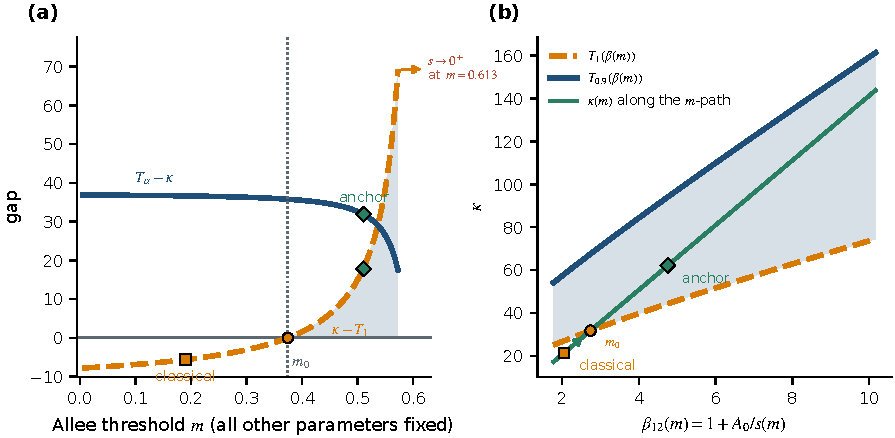
\includegraphics[width=0.95\textwidth]{fig06_double_allee_m_path.pdf}
\caption{The Allee threshold drives a fixed three-species community through exact invariant space at \(\alpha=0.9\). \textbf{(a)} Cain's gap \(\kappa-T_1\) changes sign once, at the exact crossing \(m_0=0.374451\ldots\), while \(T_{0.9}-\kappa\) remains positive on the displayed fractional-only branch. \textbf{(b)} The same path in an invariant slice. The curves use exact formulas; the marked anchor is interval-certified in Section~\ref{sec:certified}.}
\label{fig:m-path}
\end{figure}

\subsection{Exact Two- versus Three-Dimensional Ecological Contrast}

For comparison, consider the two-species model
\[
 {}^CD_t^\alpha x=x[g_{\rm DA}(x)-qy],
 \qquad
 {}^CD_t^\alpha y=y[px-d].
\]
At coexistence \(X=d/p\), the reduced matrix is
\[
 B_2=
 \begin{pmatrix}
 g_{\rm DA}'(X)&-q\\
 p&0
 \end{pmatrix}.
\]
Theorem~\ref{thm:2d} gives
\[
 B_2\in\mathcal F_\alpha^{(2)}
 \iff
 g_{\rm DA}'(X)\le0,
\]
whereas classical Hurwitz \(D\)-stability requires \(g_{\rm DA}'(X)<0\). Hence the genuinely fractional difference occurs only on the codimension-one condition
\[
 g_{\rm DA}'(X)=0.
\]
Solving this condition for the Allee threshold gives
\begin{equation}
 m_c
 =
 \frac{X^2+2aX-Ka}{K+a}.
 \label{eq:mc-2d}
\end{equation}
Thus the two-species mechanism is exceptional, while Theorem~\ref{thm:open-ecological} gives a nonempty open fractional-only region in the three-species architecture.

\section{Certified Interior Realization}\label{sec:certified}

The preceding results are analytic and do not depend on numerical sampling. We nevertheless record one certified interior realization to show that the open ecological region can be reached with nondegenerate coexistence densities and comfortable separation from both the classical and fractional boundaries.

We use \(\alpha=0.9\) and the parameter set in Table~\ref{tab:w2a}. This realization was selected from a search over constructive embeddings only after the theorem package had been fixed; the search therefore chooses a readable interior witness rather than supplying evidence for the theorem.

\begin{table}[!htbp]
\centering
\caption{Canonical certified realization W2-A. All parameters are positive; the conversion efficiencies satisfy \(0<e_1,e_2,e_3<1\).}
\label{tab:w2a}
\begin{tabular}{cccccc}
\toprule
Parameter & Value & Parameter & Value & Parameter & Value\\
\midrule
\(\alpha\) & \(0.9\) &
\(a\) & \(0.229\) &
\(K\) & \(1.4913425743\)\\
\(r\) & \(7.8104480113\) &
\(m\) & \(0.511\) &
\(h\) & \(0.1404219270\)\\
\(q_1\) & \(0.5121684678\) &
\(q_2\) & \(3.2338213736\) &
\(c_1\) & \(0.065\)\\
\(c_2\) & \(0.0509\) &
\(e_1=e_3\) & \(0.773\) &
\(e_2\) & \(0.01404592165\)\\
\(\mu_1\) & \(0.3178535346\) &
\(\mu_2\) & \(0.1209173583\) &
 & \\
\bottomrule
\end{tabular}
\end{table}

At \(m=0.511\), interval evaluation of the coexistence equations gives
\begin{equation}
 (X,Y,Z)
 =
 (1,\;0.7856328169\ldots,\;0.1921819373\ldots),
 \label{eq:w2a-densities}
\end{equation}
so the largest-to-smallest coexistence density ratio is approximately \(5.20\). The reduced prey slope and C-10 invariants are
\begin{equation}
 s=0.8231,\qquad
 \beta=(4.79,\;4.506,\;5.607),\qquad
 \kappa=62.735.
 \label{eq:w2a-invariants}
\end{equation}
The classical threshold is
\[
 T_1(\beta)
 =
 44.6123995333883\ldots,
\]
and high-precision evaluation of the unique C-15 minimizer gives
\[
 T_{0.9}(\beta)
 =
 94.5719074446105\ldots.
\]
The interval calculations certify the strict margins
\begin{equation}
 \kappa-T_1(\beta)\ge18.1226004666,
 \qquad
 T_{0.9}(\beta)-\kappa\ge31.8369074446.
 \label{eq:w2a-margins}
\end{equation}
Thus the point lies well inside the fractional-only band rather than near either boundary.

\subsection{Interval Certification along the Allee Branch}

The coexistence branch was enclosed with outward-rounded high-precision interval arithmetic. For each \(m\)-box, the scalar equilibrium equation~\eqref{eq:scalar-equilibrium} was enclosed and contracted by interval Newton evaluation; the resulting state enclosure was then propagated through \(s\), \(\beta\), \(\kappa\), and the threshold inequalities. The threshold minimizer is unique by Theorem~\ref{thm:strict-convexity}, which removes ambiguity in the exact C-10 branch used for the enclosure.

A subdivision of
\begin{equation}
 0.394\le m\le0.578
 \label{eq:certified-m-range}
\end{equation}
into 42 subintervals was certified without failure. Across this entire interval,
\[
 \kappa-T_1>0,
 \qquad
 T_{0.9}-\kappa>0.
\]
The smallest certified lower margins over the complete interval were approximately
\[
 \kappa-T_1\ge0.0332,
 \qquad
 T_{0.9}-\kappa\ge1.342.
\]
Hence Equation~\eqref{eq:certified-m-range} is a rigorous interval-certified fractional-only segment for one fixed set of non-\(m\) biological parameters.

The classical boundary itself was solved independently at high precision:
\begin{equation}
 m_0
 =
 0.37445128124251493523908034461904384927\ldots,
 \label{eq:w2a-m0}
\end{equation}
with residual below \(10^{-59}\) in the exact Cain-gap equation. This value agrees with the unique/transverse crossing predicted by Theorem~\ref{thm:crossing}.

\begin{figure}[!htbp]
\centering
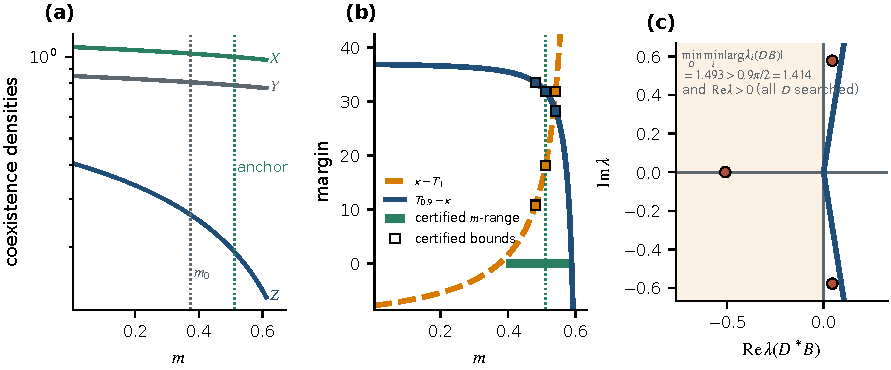
\includegraphics[width=0.95\textwidth]{fig07_certified_anchor.pdf}
\caption{Certified realization W2-A. \textbf{(a)} Positive coexistence densities along the \(m\)-branch; at the anchor, \((X,Y,Z)\approx(1,0.786,0.192)\). \textbf{(b)} Classical and fractional invariant margins; marked points and the green interval are interval-certified. \textbf{(c)} Spectrum at the most restrictive positive diagonal found by a scale-invariant angular search. Panel (c) is numerical corroboration only: the all-diagonal statement follows from Theorem~\ref{thm:c10} and the certified invariant inequalities, not from finite search.}
\label{fig:certified-anchor}
\end{figure}

\subsection{Scale-Invariant Spectral Corroboration}

As an independent numerical check, we minimized the smallest eigenvalue angle over positive diagonal ratios after fixing the geometric mean of the diagonal entries to one. This normalization is essential: raw spectral abscissa is not scale invariant under common multiplication of \(D\).

For the anchor, the most restrictive diagonal ratio found was approximately
\[
 D_*=
 \diag(0.1810,\;2.0474,\;2.6985),
\]
with eigenvalues
\[
 0.3272\pm4.2040\,i,\qquad -3.7080.
\]
Hence
\[
 \min_j|\arg\lambda_j(D_*B)|
 =
 1.49312\ldots
 >
 0.9\frac{\pi}{2},
\]
while the conjugate pair has positive real part. The corresponding angular margin is about \(0.0794\) radians for \(\alpha=0.9\), whereas the classical \(\alpha=1\) margin is negative. This direct search corroborates both sides of the classification, but it is not used in the proof.

Finally, Figure~\ref{fig:ecological-contrast} places the exact two-dimensional equality curve beside the three-dimensional open region. In panel (b), the region boundaries are traced by deterministic root finding applied to the exact formulas. The traced regions themselves are pointwise formula evaluations; only the green segment and marked anchor carry interval-certification semantics.

\begin{figure}[!htbp]
\centering
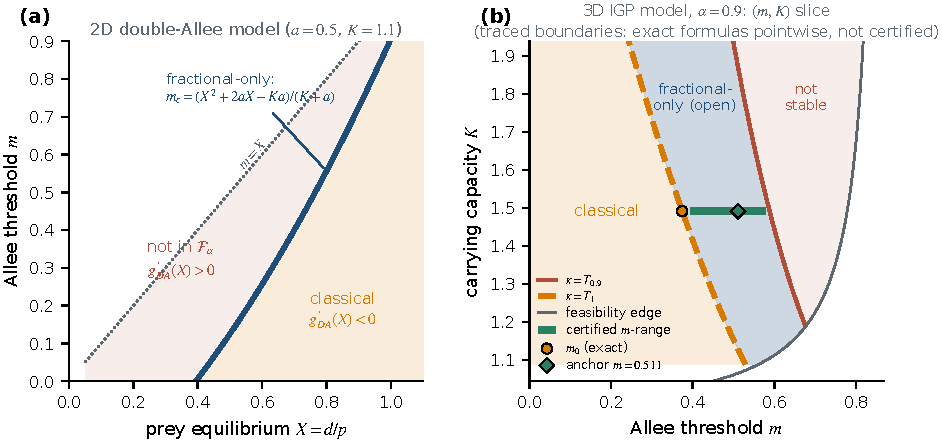
\includegraphics[width=0.96\textwidth]{fig08_double_allee_2d_3d.pdf}
\caption{Exact two- versus three-dimensional Double-Allee contrast. \textbf{(a)} In two dimensions the fractional-only class is the closed-form codimension-one curve \(m=m_c(X)\) from Equation~\eqref{eq:mc-2d}. \textbf{(b)} For the three-species W2-A design at \(\alpha=0.9\), the classical Cain boundary, Matignon boundary and feasibility edge enclose an open fractional-only region in the \((m,K)\)-plane. The green segment is interval-certified; the surrounding colored regions are deterministic evaluations of the exact formulas and are not interval certificates.}
\label{fig:ecological-contrast}
\end{figure}

\section{Discussion and Conclusions}\label{sec:discussion}

The central distinction in this paper is between stability of one Jacobian and robustness of its complete positive-diagonal orbit. For a fixed commensurate Caputo linearization, the Matignon sector can admit a right-half-plane conjugate pair \cite{Matignon1996,BrandiburGarrappaKaslik2021}. Here the stronger statement is that the \emph{linearized Jacobian} remains Matignon-stable after every positive diagonal left scaling, even when the same orbit is not classically Hurwitz \(D\)-stable. Classical ecological \(D\)-stability is already a recognized robustness concept \cite{ChenWangLiu2024}; our contribution is the exact three-dimensional Matignon deformation of Cain's boundary and its nonlinear ecological realization.

The dimension statement must also be read precisely. Dimension three is not the first dimension in which fractional stabilization can occur. It is the minimum dimension in which
\[
\mathcal F_\alpha^{(n)}\setminus\mathcal D_H^{(n)}
\]
has nonempty full-dimensional interior. In two dimensions the difference class is confined to an equality locus; in three dimensions the exact interval \(T_1(\beta)<\kappa<T_\alpha(\beta)\) is open. The strict-convexity result makes this boundary computationally and analytically well behaved: the threshold has a unique nondegenerate optimizer and varies smoothly with the invariant coordinates.

The ecological construction gives the invariant geometry a mechanistic interpretation without claiming novelty for IGP or Allee ecology. In the two-consumer architecture the directed three-cycle term has the sign that forces \(\kappa<T_1\), so parameter tuning cannot reach the fractional-only band. In the IGP architecture one cycle changes sign and makes \(L_3<0\) accessible. The resulting four-invariant right inverse, followed by the Double-Allee embedding, yields a nonempty open subset of the full 14-dimensional positive biological parameter space for each fixed \(\alpha\). Along that branch the Allee threshold has an exact matrix-geometric role: increasing \(m\) decreases \(s=-g'_{\rm DA}(X)\), so \(t=1/s\) increases and can cross Cain's surface uniquely and transversally while all other biological parameters remain fixed.

The scope is local and spectral. Membership in \(\mathcal F_\alpha\) concerns the linearized commensurate Caputo system; it does not prove global nonlinear stability, a Hopf bifurcation, or global uniqueness of positive coexistence. The constructed equilibrium is a smooth local branch. The W2-A realization is a biologically feasible mathematical witness with certified margins, not an empirical calibration, and the direct diagonal search in Section~\ref{sec:certified} is corroboration rather than proof.

In summary, the universal positive-diagonal quantifier for real \(3\times3\) matrices on the strict-\(P(-A)\) stratum reduces exactly to
\[
\kappa<T_\alpha(\beta).
\]
The threshold recovers Cain at \(\alpha=1\), lies strictly above it for \(\alpha<1\), and has a unique smooth optimizer. This yields the minimum full-dimensional robust dimension \(n=3\). A nonlinear Caputo Double-Allee IGP system then realizes an open subset of the resulting fractional-only class, while the competing-consumer architecture is structurally excluded and the Allee threshold supplies an exact crossing mechanism. For \(n\ge4\), the simplex reduction remains available but the number of nontrivial orbit invariants grows to \(2^n-n-1\); identifying higher-dimensional graph classes that retain comparable low-dimensional structure is the natural next problem.


\authorcontributions{Conceptualization, I.A. and T.N.A.; methodology, I.A. and T.N.A.; formal analysis, I.A. and T.N.A.; verification software, I.A.; writing---original draft, I.A.; writing---review and editing, I.A. and T.N.A. All authors have read and agreed to the submitted version of the manuscript.}

\funding{This research received no external funding.}

\dataavailability{The analytical derivations and the numerical values required to assess the claims are contained in the article. Reproducibility scripts were used for internal verification; no external dataset or supplementary material is required for the results.}

\acknowledgments{The authors are thankful to the Deanship of Graduate Studies and Scientific Research at University of Bisha for supporting this work through the Fast-Track Research Support Program.}

\conflictsofinterest{The authors declare no conflicts of interest.}

\begin{adjustwidth}{-\extralength}{0cm}
\reftitle{References}
\bibliographystyle{../reference-paper/Definitions/mdpi}
\bibliography{references}
\end{adjustwidth}

\end{document}
